\chapter{Introduction and Overview}

\section{Active electro-location}

\label{sec:presentation_poisson}

This section will be devoted to the fish itself. After a short
presentation (living conditions, species, etc.) the
electro-location aspects will be emphasized:~organs involved in
the generation and the acquisition of the electric field,
experimental evidence and performance of this ability, behavior
observed while hunting. At the end, a short review of the efforts
made to simulate this phenomenon will be given.

These lines rely mainly on two complete and well documented books:
the first one is written by Peter Moller
\noun{\cite{moller1995electric}} and the second, published more
recently, was made in collaboration by the main specialists of the
subject \cite{bullock2005electroreception}.


\subsection{Taxonomy and living conditions}

There are dozens of weakly electric species, classified in various
families. These families all belong to two different orders: Gymnotiforms
in South America and Mormyriforms in Africa (see Figure \ref{fig:geography}).
%
\begin{figure}[!h]
 \centering 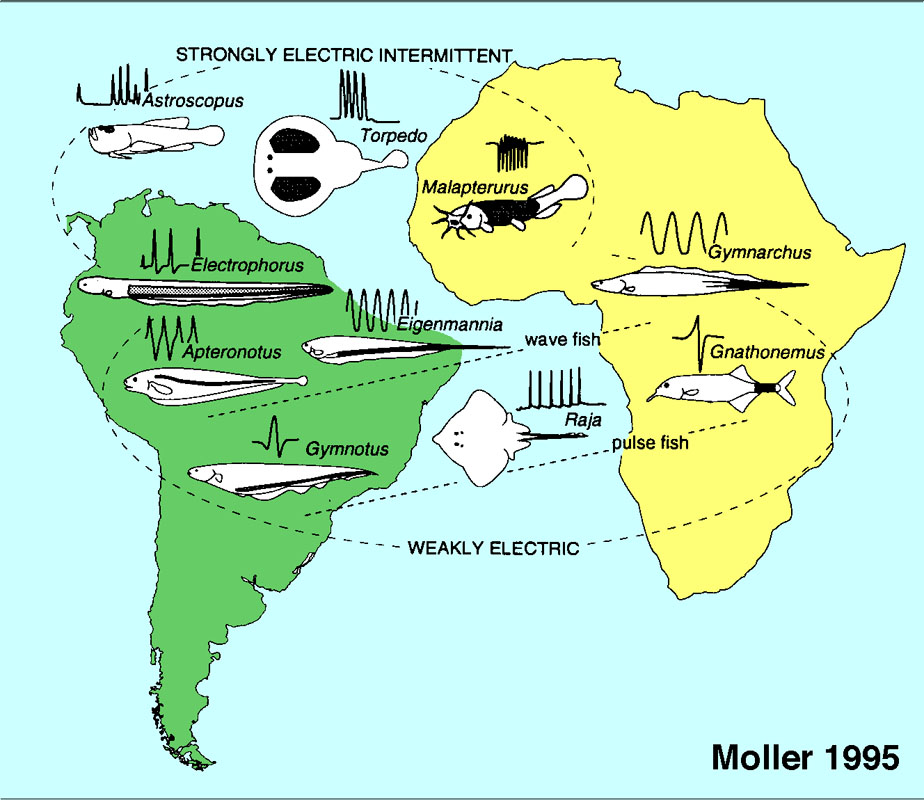
\includegraphics[width=10cm]{fish_geography} \caption{Classification and geographic distribution
 of the different species
of weakly electric fish. The species of interest are in the lower
circle and the other ones use their electric organ in an
aggressive or defensive manner. Taken
from~\cite{moller1995electric}. \label{fig:geography}}

\end{figure}


These fishes live in muddy rivers, hunt at night and sleep during
the day. Their shape and size vary considerably from one specie to
another. Two types are distinguished according to the electric signal
emitted: pulse-type species and wave-type species (see Figure \ref{fig:pulse_wave}).
%
\begin{figure}[!h]
 \centering 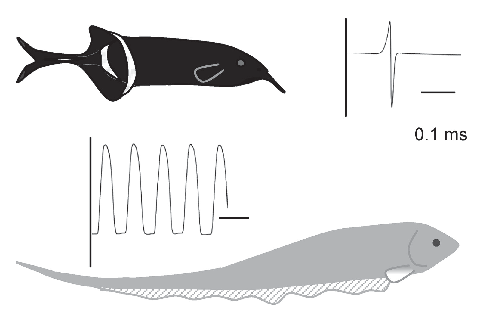
\includegraphics[width=13cm]{pulse_wave} \caption{Differences betweend two species: one
 is pulse-type (on the left)
and the other is wave-type. For each on, its electric discharge is
represented in time scale (exterior graphics) and in frequency scale
(interior graphics). Taken from \cite{heiligenberg1991neural}. \label{fig:pulse_wave}}

\end{figure}



\subsection{Emitting and receiving the electric field}

This section will explain the physical, chemical and biological mechanisms
involved during \emph{electrogenesis} and \emph{electroreception}.

Whatever the type of specie (wave or pulse), the emission relies on
the same principle and is due to a specific organ which is generally
situated in the tail;~the first paragraph will provide more details.
The reception is operated by receptors spreading on the surface of
the skin; further explanation will be given in a second time.


\subsubsection*{The electric organ}

Apart from the family Apteronotidae (in the Gymnotiforms order), the
Electric Organ (denoted EO below) emitting the electric discharges
derives from muscular tissues - it is called \emph{myogenic organ}
- built in superimposed disks (cf Figure \ref{fig:electric_organ}).
These disks are in fact big cells ($0.75$ mm in \emph{Brachyhypopomus
pinnicaudatus} \cite{stoddard2008signal}) called \emph{electrocytes.}
Their number ranges from hundreds (in Mormyrids) to several millions
in strongly electric species.%
\begin{figure}[!h]
 \centering 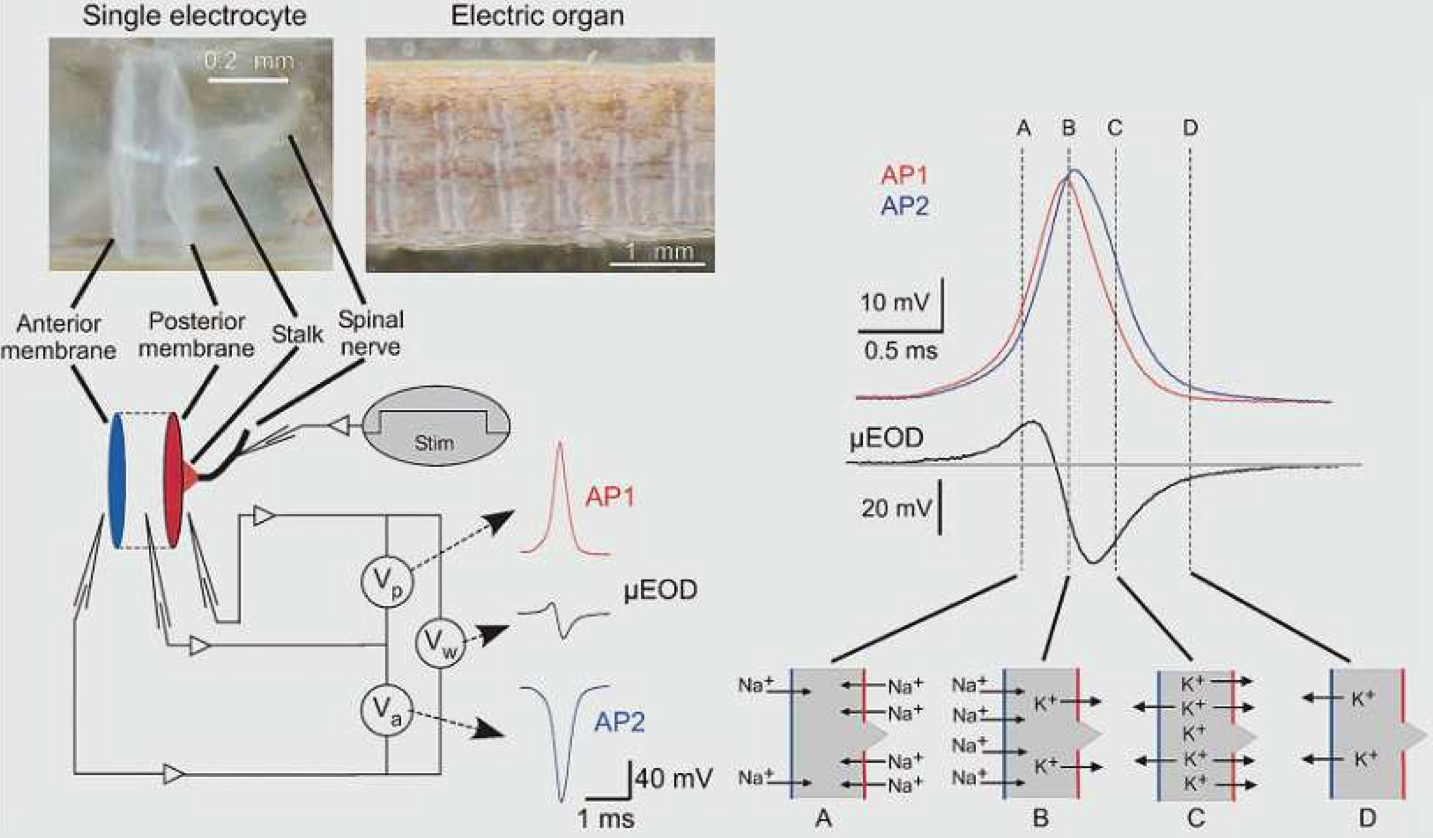
\includegraphics[width=12cm]{electric_organ} \caption{A \emph{Brachyhypopomus pinnicaudatus}
 electrocyte. Taken from \cite{stoddard2008signal}.
\label{fig:electric_organ}}

\end{figure}


An \emph{Electric Organ Discharge} (denoted EOD below) is as follows:
first, the brain sends an impulse that goes through a pacemaker in
the spinal cord. This pacemaker is connected to every electrocyte
by a \emph{spinal nerve}. Each nerve depolarizes the caudal (\emph{i.e.}
posterior) part of the cell, which causes the opening of the ionic
canals situated on the membrane (they are uniquely sensible to voltage
difference between the interior and the exterior of the cell). It
follows a ionic flux (see A, B, C and D in Figure \ref{fig:electric_organ})
that makes the electric current. It should be noted that the great
similarity with a battery is historic: indeed, \noun{Volta} built
its first pile in 1800 according to his observations of the eel's
organ \cite{volta1800} and named it \emph{Artificial Electric Organ}.

However, in Apteronotidae species the EO derives from neural tissues
and therefore is said to be \emph{neurogenic}. In this case, the organ
is composed of several presynaptic axons of electromotor nerves (see
Figure \ref{fig:neurone}) that are not connected at their end. When
the brain sends a signal in these neurons, the sum of all the small
currents makes the discharge.

%
\begin{figure}
\centering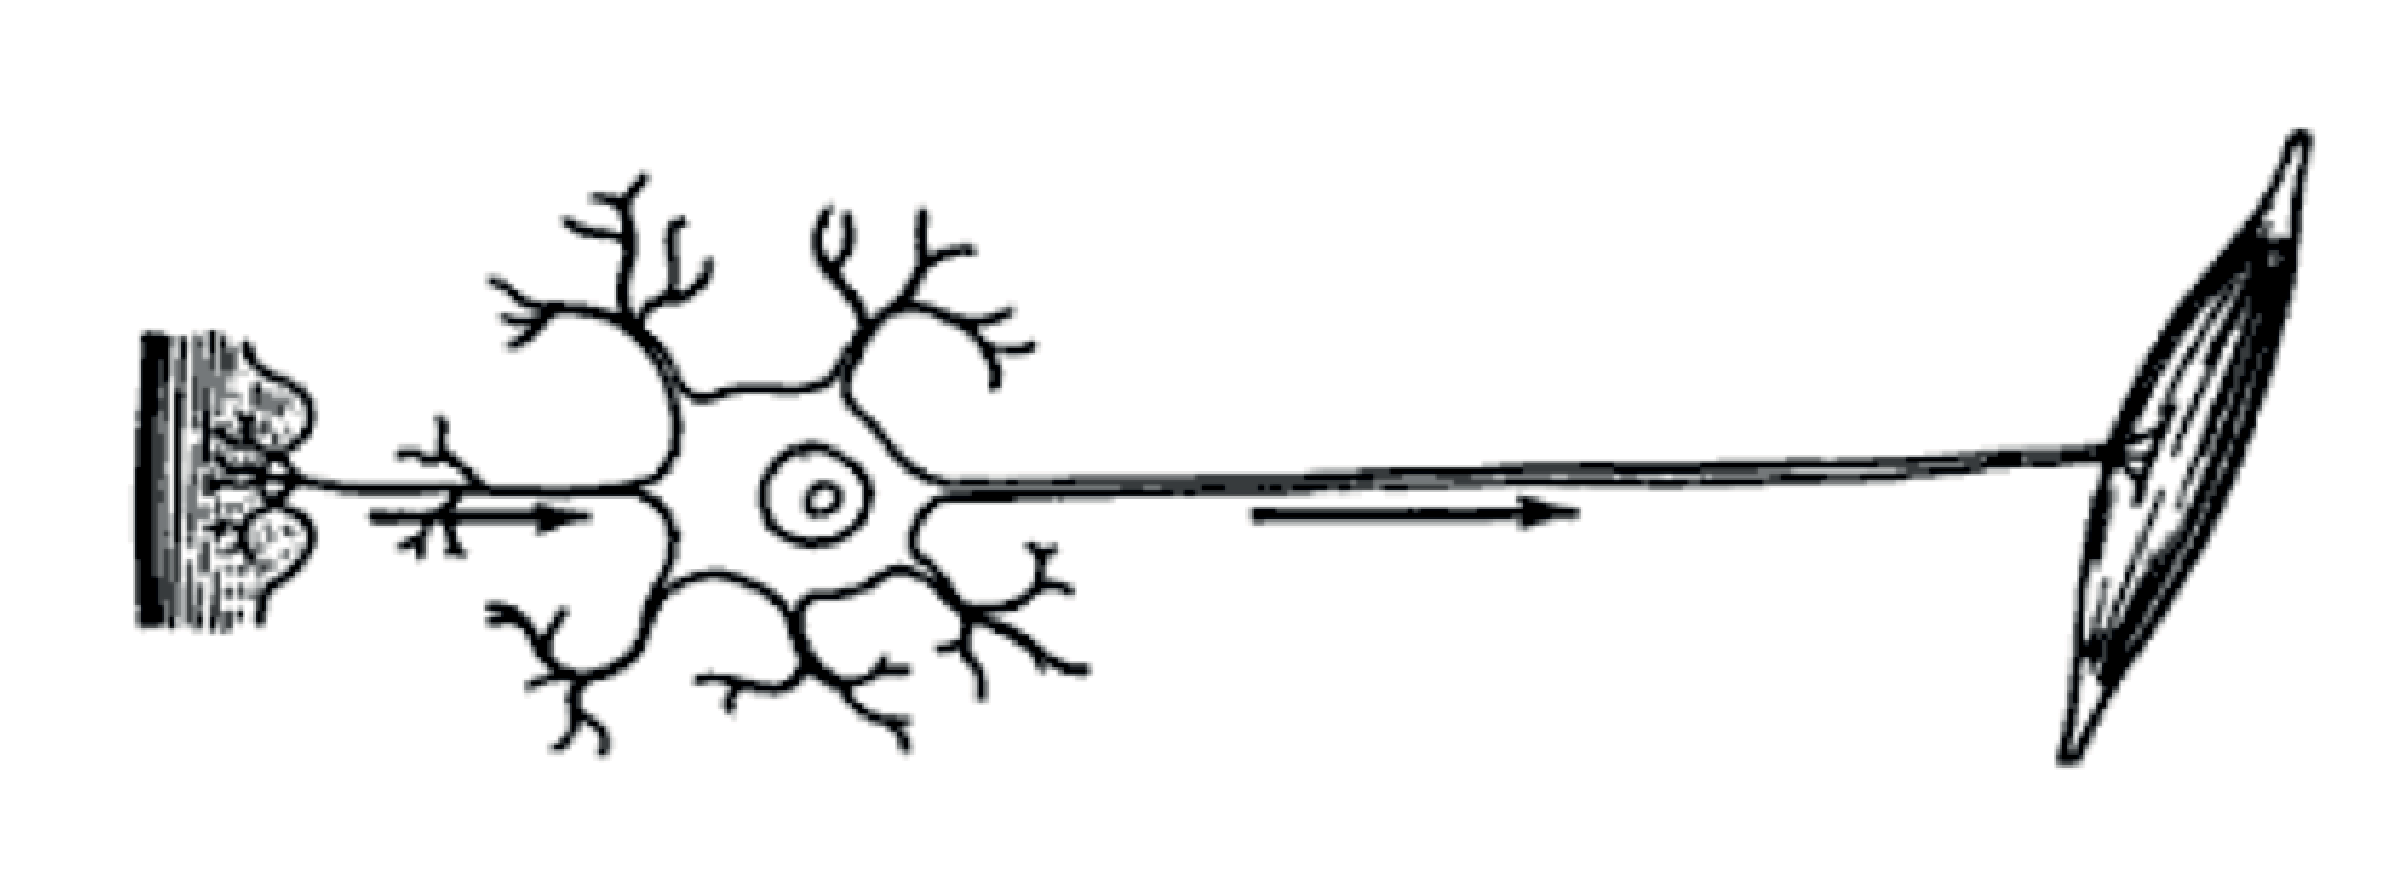
\includegraphics[width=7cm]{neurone}

\caption{An electromotor neuron. The axon connects the body of the neuron (in
the center) to the muscular tissues (on the right). Taken from \cite{rouviere2002}.
\label{fig:neurone}}

\end{figure}


Depending on the species, this organ occupies a small part of the
body (for example in Mormyrids it is located in the caudal peduncle)
or an extended one (for example almost the entire trunk in \emph{Gymnarchus
niloticus}).


\subsubsection*{Electroreceptors}

\label{sub:electrorecepteurs}

There are thousands of pores - sizing around a millimeter - on its
scaleless skin. In each of them can be found an electroreceptor
used to measure the voltage difference between the exterior medium
and the inside of the fish's body. A receptor is formed by a
cavity filled by a conducting material (liquid or fibers): when a
potential difference is applied a current appears in this
material, which is measured by sensitive cells (see Figure
\ref{fig:electroreceptor}). Then this information is transmitted
to the brain via \emph{afferent neurons}.

Two types of receptors are distinguished according to their shape:
\emph{ampullary} receptors and \emph{tuberous} ones. The shape is
not the only difference, since the ampullary receptors measure low
frequency signals (from $1$ to $10$ Hertz) and the others are
sensitive to high frequencies (from a hundred of Hertz to $1$
kiloHertz). Moreover, the laters can be either sensitive to the
amplitude of the signal (in this case they are called AM for
\emph{Amplitude-Modulating units}) or to the frequency (here they
are called RT for \emph{Rapid Timing
units}). %
\begin{figure}[h]
 \centering 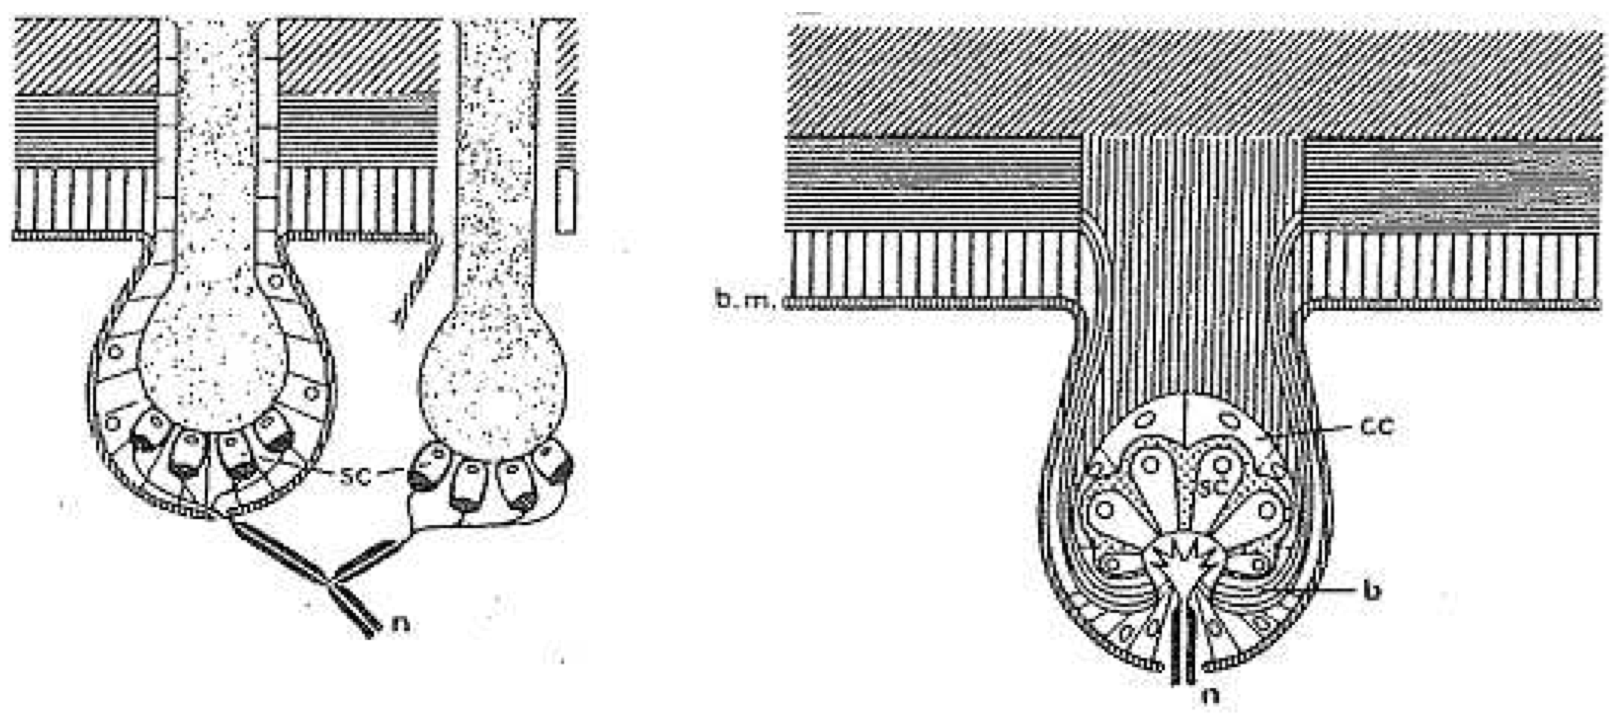
\includegraphics[width=10cm]{electroreceptors} \caption{Two types of electroreceptors:
 an ampullary receptor on the left (this
shape is common to Mormyrids and Gymnotiforms) and a tuberous one
on the right (this shape of organ is from Gymnotiforms). Sensitive
cells are indicated by {}``sc'' and the afferent neurons are noted
{}``n''. Taken from \cite{moller1995electric}. \label{fig:electroreceptor}}

\end{figure}


However the repartition on the skin depends on the species, there
are similarities in each order. Indeed, it is rather uniform in Gymnotiforms
(though the density is higher near the head) and it is concentrated
on the back and on the ventral part of the body in Mormyriforms (see
Figure~\ref{fig:density_electroreceptor}). %
\begin{figure}[h]
 \centering 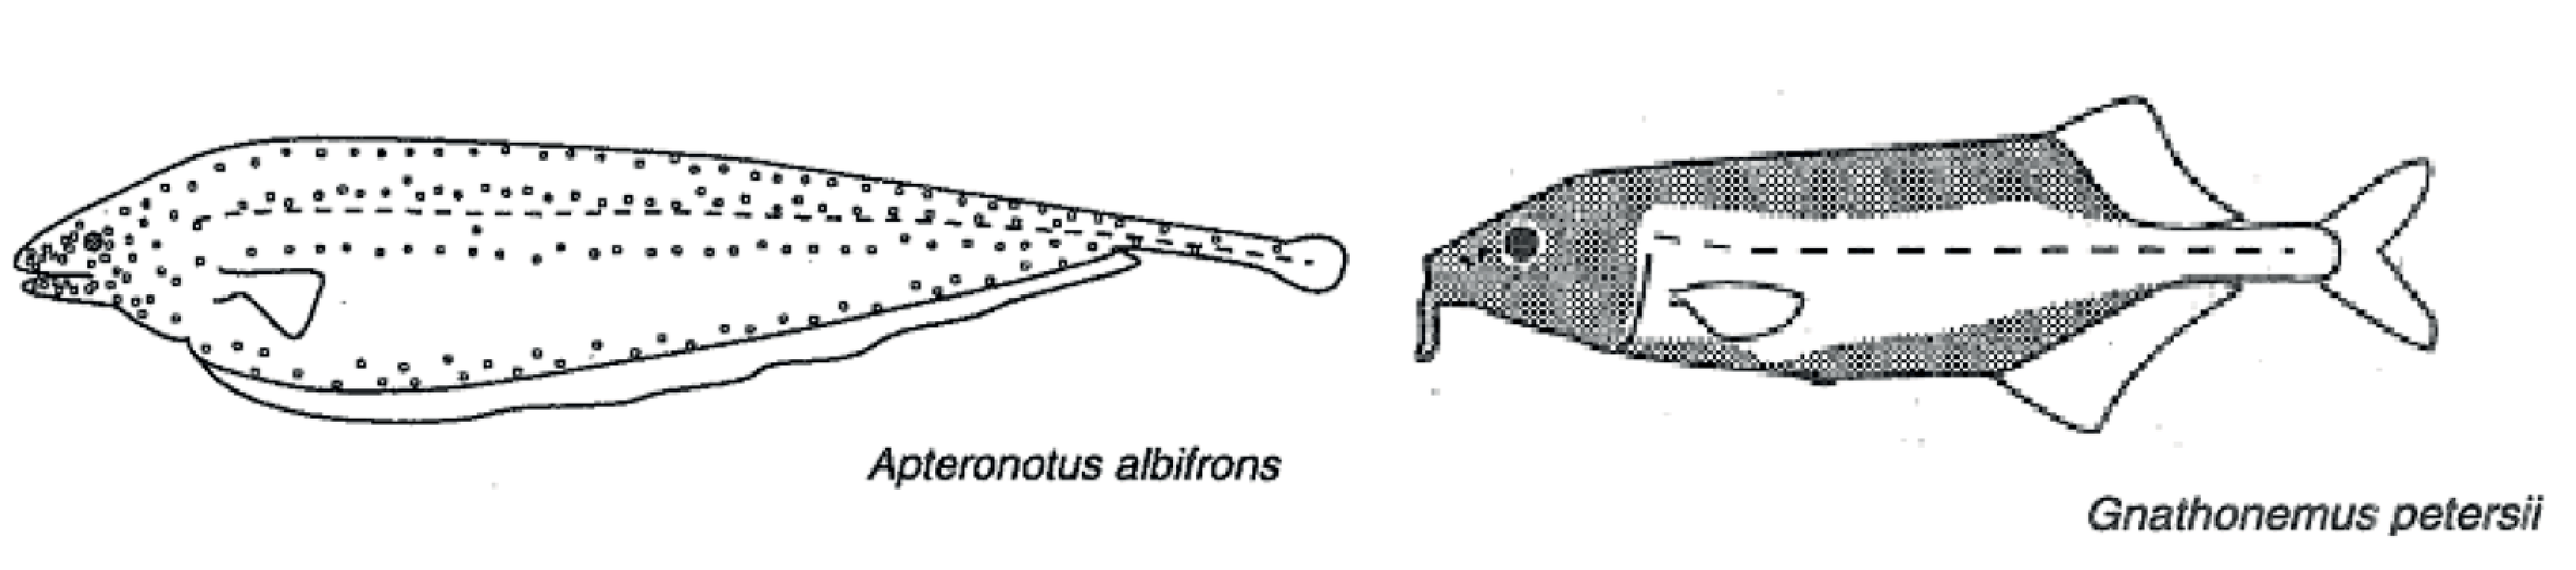
\includegraphics[width=10cm]{density_electroreceptors}
\caption{Location of the receptors according to the order: \emph{A. albifrons}
is a Gymnotiform (each dot represents an ampullary organ - the tuberous
ones show the same repartition but are simply in a higher number)
and \emph{G. petersii} belongs to the Mormyrifoms order (the receptors
are situated in the shaded area). Taken from \cite{moller1995electric}.
\label{fig:density_electroreceptor}}

\end{figure}



\subsection{Electro-location: behavior and performance}

\label{sub:electro-localisation}

These fishes live in turbid water, mostly at night, and hunt small
preys - like insects or small fishes
\cite{albert2005diversity,okedi1971food}. The vision is useless in
these conditions and they rely mainly on their electric sense. Two
behaviors are to be described in this section: \emph{passive
}electro-location and \emph{active }electro-location.


\subsubsection*{Passive electro-location}

This type of detection is not exclusive to weakly electric fish:
for example sharks and rays also use it
\cite{adair1998detection,kalmijn-1988}. From the point of view of
evolution, it seems to be anterior to active electro-location
\cite{lissmann1958evolution}. It is based on the detection of the
low frequencies of the electric field emitted by external sources
(physical, chemical or biological \cite{kalmijn-1988}).
Experimentally, it can be observed when the fish is in the field
of an electric dipole \cite{hopkins-passive}: it tends to align
its body with the streamlines and to follow it until the source
(see Figure \ref{fig:behavior_passive_electro-location}).
Consequently, this behavior does not involve a complex analysis of
the electric field and the fish does not seem to know by advance
where is the dipole. Since it is well understood, we will not
study it.

%
\begin{figure}[h]
 \centering\includegraphics[width=10cm]{behavior_passive_electro-location}

\caption{Behavior of \emph{G. carapo} in the presence of a dipole,
with two different geometries. Full lines correspond to pathway
followed by the fish during an essay ($N$ is the number of essays)
and doted lines are stremlines of the electric field. Taken
from~\cite{davis1988behavioural}.\label{fig:behavior_passive_electro-location}}

\end{figure}



\subsubsection*{Active electro-location}

Active electro-location is far more complex because the fish seems
to know away from the object its location and its properties. It
has long been known that weakly electric fishes react strongly
when a
metallic rod enters the aquarium %
\footnote{in fact since the XVIII$^{th}$ century, when electrogenesis is discovered
\cite{moller1995electric}%
}. But it took centuries to understand why: in 1958, Hans Lissmann
finally connected this fact with their emission of a weak electric
field and concluded that they possess an {}``electric sense''.
This sense has a range of about one or two body length. Behavioral
studies showed that these fishes are able to determine the
distance (Figure \ref{fig:distance_discrimination}A), the size,
the shape (Figure \ref{fig:distance_discrimination}B) and the
material (via resistivity and capacitance) of an object
\cite{von1999active,von1992electro-location,von1993electric}.

%
\begin{figure}[h]
 \centering\includegraphics[width=12cm]{distance_discrimination}

\caption{(A) Experimental evidence of distance measurement by a
\emph{Gnathonemus petersii}. On the left: experimental setup. The
fish is forced to enter one of two gates where objects $S^{+}$ and
$S^{-}$ are placed. These objects only differ by their distance
$D$ with respect to the gate. If the first one is chosen, the fish
is rewarded (by feeding) and if not, the fish is punished (by
disturbing it). On the right is plotted the rate of correct choice
as a function of $D$. The objects $S^{+}$ and $S^{-}$ are metallic
sphere with a volume of $33.5$
cm$^{3}$. (Taken from \cite{von1993electric}). \protect \\
 (B) Experimental evidence of shape discrimination by individuals
of the same specie. The experimental setup is the same, except
that the difference between the objects is now their shape: one is
a metallic cube whereas the other is a metallic cylinder. (Taken
from \cite{von2004distance}). \label{fig:distance_discrimination}}

\end{figure}


The physical principle of electro-location has been known since
its discovery by \noun{Lissmann} in 1958
\cite{lissmann1958mechanism}: the electric field's amplitude and
frequency are modified when there is an element in the surrounding
with conductivity and capacitance - respectively - different from
that of the water. This modification is then felt by tuberous
receptors all over the skin and the fish analyzes this data.
However, no one knows an algorithm that can translate this data
into information on the object.

It should be noticed that when the fish probes its environment, is
exhibits an intense activity \cite{lannoo1993electric}. Moreover,
the swimming patterns are quite uncommon. For example,
Gymnotiforms do not have caudal nor dorsal fin so swimming depends
entirely on their anal fin; the result is that they can swim
either forward or backward without difficulty. The strategy used
during exploration has been called \emph{Probing Motor Acts} by
Toerring\noun{ and }Belbenoit~\cite{toerring1979motor}:~see
Figure~\ref{fig:pma}. %
\begin{figure}[h]
 \centering \includegraphics[width=12cm]{pma} \caption{PMA: behavior exhibited by mormyrids (\emph{Marcusenius
 cyprinoides
}and \emph{Gnathonemus petersii}) when introducing a metallic - or
plastic - object (showed by the black dot). 1.~chin probing 2a.~lateral
{}``va-et-vient'' 2b.~radial {}``va-et-vient'' 3.~lateral probing
4.~tangential probing 5.~stationary probing. Taken from \cite{toerring1984locomotor}.\label{fig:pma}}

\end{figure}


During the exploration, pulse-type species control the EOD rate by
stabilizing the frequency (see Figure
\ref{fig:EOD_stabilization}). In both types, an amplitude
enhancement is also observed. A special care will be made on these
strategies when modelling the problem.

%
\begin{figure}[h]
 \centering\includegraphics[width=10cm]{EOD_stabilization}

\caption{EOD rate as a function of the fish's activity. Taken from \cite{toerring1984locomotor}.
\label{fig:EOD_stabilization}}

\end{figure}



\subsection{Modelling the electric field}

\label{sub:modelisation_champ_bio}

Electro-location has been quantitatively investigated since it is
known: in their article, Lissmann and Machin tried an analytical
approach by calculating the distortion of a dipole's electric
field caused by an infinite cylinder \cite{lissmann1958mechanism}.
This section will give a brief state-of-the-art of the progress
that has been made since then. First, we will focus on analytical
results, and various numerical approaches of the electric field
will follow.

Formulas have been established to compute the effect of a scatterer
in the fish's field by several authors: Lissmann and Machin in 1958
\cite{lissmann1958mechanism}, Bacher in 1983 \cite{bacher1983} and
Rasnow in 1996 \cite{rasnow1996simple}. All of them rely on the fact
that a sphere placed in a uniform electric field {}``creates'' another
field equivalent to a dipole's one. Let us see in detail what are
these formulas. In the first article, an infinite cylinder with conductivity
$\sigma$ is illuminated in a medium of conductivity $\sigma_{0}$
by a dipole $M$. In the plane, the equivalent dipole $M'$ of the
cylinder is given by the following expression (with the notations
of Figure \ref{fig:modele_lissmann}):

\begin{equation}
\frac{M'}{M}=a^{2}\left(\frac{\sigma_{0}-\sigma}{\sigma_{0}+\sigma}\right)\frac{1}{r_{1}r_{2}}\label{eq:dipole_lissmann}\end{equation}


%
\begin{figure}
\centering\includegraphics[width=9cm]{dipole_lissmann}

\caption{Model used by Lissmann and Machin. An infinite cylinder of radius
$a$ is in the neighborhood of a dipole formed by two sources $+q$
and $-q$ which are separated by a distance $l$. Taken from \cite{lissmann1958mechanism}.
\label{fig:modele_lissmann}}

\end{figure}


In 1983, Bacher remarks that this formula cannot explain the phase
difference observed when the electric permittivity of the target
does not equal the water's permittivity \cite{bacher1983}. This
phase difference is important since it is measured by RT units
receptors (see section~\ref{sub:electrorecepteurs}). He proposes
then to take this into account in the equations by considering a
non-stationary electric field, but does not give a formula similar
to (\ref{eq:dipole_lissmann}). Rasnow resolves this problem in
1996 by considering a harmonic regime for the background electric
field: in the presence of a sphere of radius $a$, conductivity
$\sigma_{1}$ and permittivity $\varepsilon_{1}$, a uniform
harmonic electric field $E_{0}$ with frequency $\omega$ is
modified in this way:\begin{equation} \delta
u(\boldsymbol{r})=\boldsymbol{E_{0}}\cdot\boldsymbol{r}\left(\frac{a}{r}\right)^{3}\frac{\left(\sigma_{1}
+i\omega\varepsilon_{1}\right)-\left(\sigma_{0}+i\omega\varepsilon_{0}\right)}{2\left(\sigma_{1}+i\omega\varepsilon_{1}\right)+\left(\sigma_{0}+i\omega\varepsilon_{0}\right)},\label{eq:dipole_rasnow}\end{equation}
where the indices $0$ refers to the ambient medium. As we will see
in section \ref{sub:D=00003D0000E9veloppements-asymptotiques}, it
corresponds to the first order approximation of the potential $u$
that verifies the equation
$-\nabla\cdot(\sigma+i\omega\varepsilon)\nabla u=0$ where $\sigma$
(resp. $\varepsilon$) is equal to $\sigma_{1}$ (resp.
$\varepsilon_{1}$) in the sphere and $\sigma_{0}$ (resp.
$\varepsilon_{0}$) in the exterior. Let us remark that the factor
in the formula (\ref{eq:dipole_rasnow}) is opposed to the one in
(\ref{eq:dipole_lissmann}) because the vector $\boldsymbol{r}$
does not point at the same direction, and the factor $2$ in the
denominator is due to the fact that we are now in the whole space
and not only in the plane (see section
\ref{sub:D=00003D0000E9veloppements-asymptotiques},
formula~\ref{eq:tenseur_polarisation_sphere}). However the model
has been improved, it is only correct in an ideal case: the target
is a sphere and the field is supposed to be uniform. It is not
reasonable because for example the latter assumption is not true
around the tail \cite{assad1998electric,assad1999electric}. The
next section will show how the tools developed recently in
mathematical imaging can handle it.

Numerical approaches have also been made since the 70's: in 1975,
Heiligenberg proposes a finite differences scheme to calculate the
field created by the fish \cite{heiligenberg1975theoretical}. In
1980, Hoshimiya\noun{ }et al. use finite elements to solve this problem
\cite{hoshimiya1980theapteronotus}. The geometry of the fish is simplified
by an ellipse and is divided into two areas: the thin skin with low
conductivity and the inside of the body. Their aim is to optimize
conductivity values to approximate as well as possible the experimentally
measured field. The result is that the optimal conductivity is non-uniform,
being higher in the tail region (see Figure \ref{fig:skin_resistance_hoshimiya}).

%
\begin{figure}
\centering\includegraphics[width=7cm]{skin_resistance_hoshimiya}

\caption{Optimal repartition of the ratio between skin resistivity $\rho_{s}$
and body conductivity $\rho_{f}$ along the head-tail axis. Taken
from~\cite{hoshimiya1980theapteronotus}. \label{fig:skin_resistance_hoshimiya}}

\end{figure}


A lot of improvement has been made since this study (see for
example
\cite{babineau2006modeling,maciver2001computational,migliaro2005theoretical,rasnow1989simulation}).
It is know well-accepted that the skin conductivity is not uniform
(higher in the head) but remains low with regards to the water
conductivity, and that the body conductivity is high. According to
Migliaro et al.\noun{ }\cite{migliaro2005theoretical}, the first
fact increases the sensitivity of the skin by enhancing the
voltage difference and the second extends and makes uniform the
potential near the skin (which is indeed experimentally measured
\cite{nelson-target}). The relative error between measures and
simulations is around $10$\%.

Another promising technique is the use of the boundary elements
method performed by Chris Assad in 1997 \cite{assad1997phd}.
Indeed the important feature is the electric potential on the skin
(because it is the \emph{input} for the fish), so a BEM approach
allows us to concentrate the equations on it. Moreover, the speed
of calculation is enhanced because the number of nodes is
dramatically reduced. The equation considered is here $\Delta u=0$
on the exterior of the body with Robin boundary conditions on the
skin~\cite{williams1990hypercube}:\begin{equation}
u-\xi\frac{\partial u}{\partial
n}=\psi,\label{eq:CL_assad}\end{equation} where $\psi$ is the
potential inside the body and
$\xi=h\left(\sigma_{0}/\sigma_{s}\right)$ ($h$ being the skin
thickness, $\sigma_{s}$ the skin conductivity and $\sigma_{0}$ the
water conductivity) is the \emph{effective skin thickness}. In the
next section we will show the validity of this model, which
permits us to easily simulate the PMA: see
Figure~\ref{fig:simulation_bem_assad}.

%
\begin{figure}
\centering\includegraphics[width=10cm]{simulation_BEM_Assad}

\caption{BEM simulation of the field with an object, the fish's
body being curved. Isopotentials are depicted by lines ($1$ mV
between each one) and the normalized arrows indicate streamlines.
Taken from \cite{assad1998electric}.
\label{fig:simulation_bem_assad}}

\end{figure}


Let us notice that there are other kind of simulations, based on a
more empirical approach, determining an equivalent electric
circuit \cite{budelli2000electric,caputi1998electric} or an
equivalent multipole \cite{chen2005modeling}.

To conclude this section, we have seen that weakly electric fish are
able to collect data issued from their self-generated electric field,
and to analyze them in order to determine features of scatterers around
them. So far, numerical studies have been made to compute this electric
field but with a lot of differences in their approaches. Our goal
here is to analyze quantitatively the equations in order to have a
precise forward problem.

\section{Outline of the Research Work}

This section briefly presents what has been done during my PhD thesis.